\documentclass{standalone}
\usepackage{tikz}
\usetikzlibrary{patterns, positioning}


\begin{document}
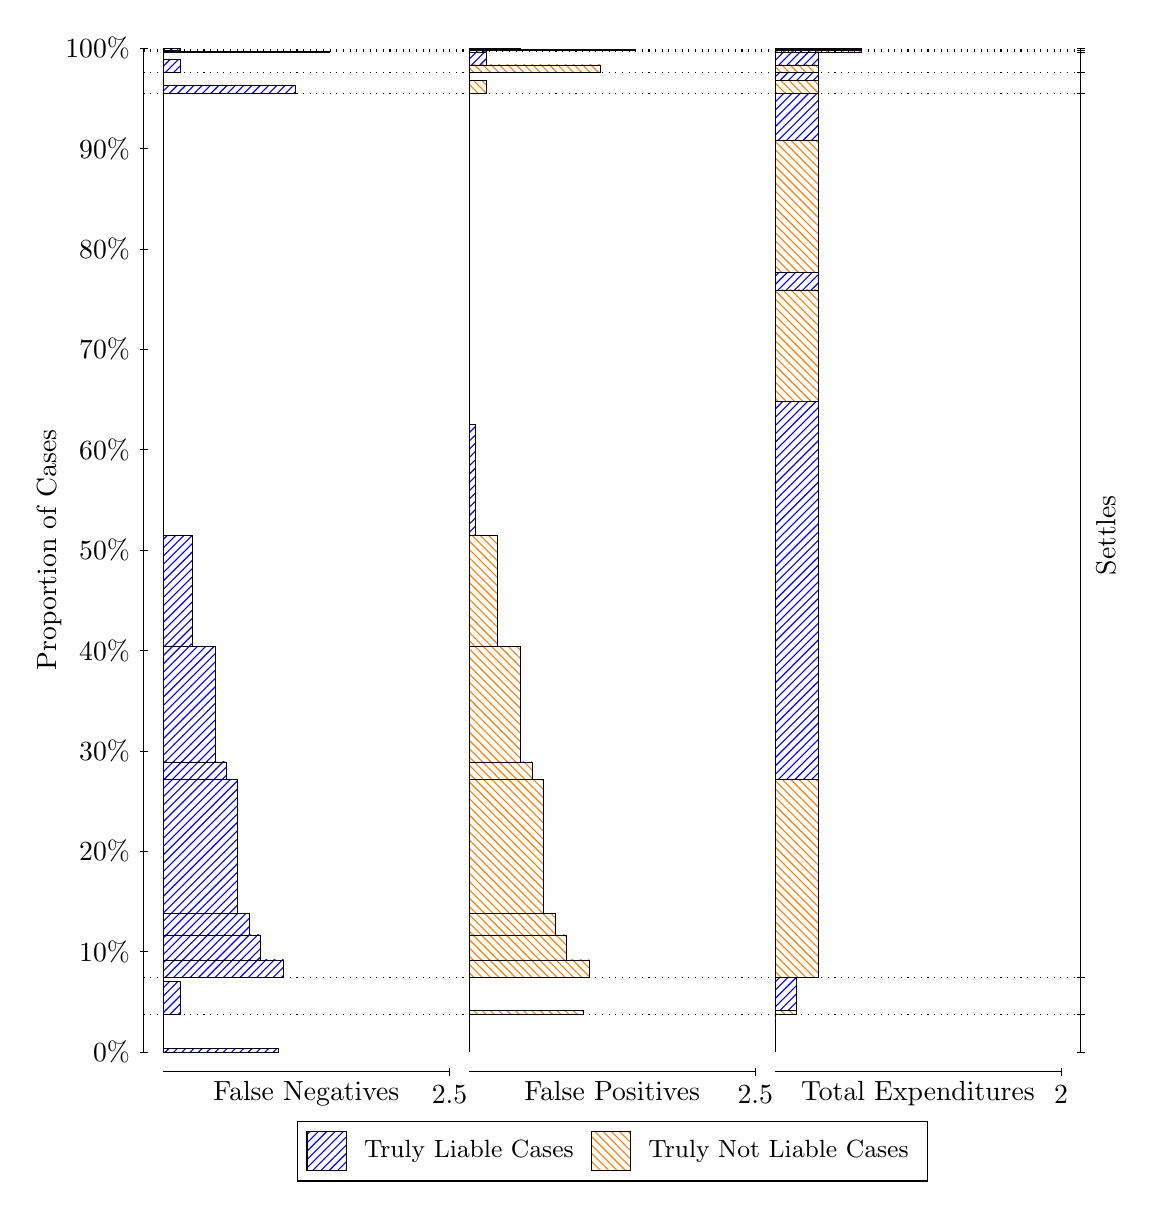
\begin{tikzpicture}
\draw[black, very thin] (1.5,1.75) -- (1.5,14.5);
\node[rotate=90, text=black, anchor=center] at (0.3, 8.125) {Proportion of Cases};
\draw[black, very thin] (1.45,1.75) -- (1.55,1.75);
\node[text=black, anchor=east] at (1.45, 1.75) {0\%};
\draw[black, very thin] (1.45,3.025) -- (1.55,3.025);
\node[text=black, anchor=east] at (1.45, 3.025) {10\%};
\draw[black, very thin] (1.45,4.3) -- (1.55,4.3);
\node[text=black, anchor=east] at (1.45, 4.3) {20\%};
\draw[black, very thin] (1.45,5.575) -- (1.55,5.575);
\node[text=black, anchor=east] at (1.45, 5.575) {30\%};
\draw[black, very thin] (1.45,6.85) -- (1.55,6.85);
\node[text=black, anchor=east] at (1.45, 6.85) {40\%};
\draw[black, very thin] (1.45,8.125) -- (1.55,8.125);
\node[text=black, anchor=east] at (1.45, 8.125) {50\%};
\draw[black, very thin] (1.45,9.4) -- (1.55,9.4);
\node[text=black, anchor=east] at (1.45, 9.4) {60\%};
\draw[black, very thin] (1.45,10.675) -- (1.55,10.675);
\node[text=black, anchor=east] at (1.45, 10.675) {70\%};
\draw[black, very thin] (1.45,11.95) -- (1.55,11.95);
\node[text=black, anchor=east] at (1.45, 11.95) {80\%};
\draw[black, very thin] (1.45,13.225) -- (1.55,13.225);
\node[text=black, anchor=east] at (1.45, 13.225) {90\%};
\draw[black, very thin] (1.45,14.5) -- (1.55,14.5);
\node[text=black, anchor=east] at (1.45, 14.5) {100\%};

\draw[black, very thin] (13.4,1.75) -- (13.4,14.5);
\draw[black, very thin] (13.35,1.75) -- (13.45,1.75);
\node[anchor=west] at (13.35, 1.75) {};
\draw[black, very thin] (13.35,2.2245) -- (13.45,2.2245);
\node[anchor=west] at (13.35, 2.2245) {};
\draw[black, very thin] (13.35,2.6989) -- (13.45,2.6989);
\node[anchor=west] at (13.35, 2.6989) {};
\draw[black, very thin] (13.35,13.924) -- (13.45,13.924);
\node[anchor=west] at (13.35, 13.924) {};
\draw[black, very thin] (13.35,14.188) -- (13.45,14.188);
\node[anchor=west] at (13.35, 14.188) {};
\draw[black, very thin] (13.35,14.451) -- (13.45,14.451);
\node[anchor=west] at (13.35, 14.451) {};
\draw[black, very thin] (13.35,14.475) -- (13.45,14.475);
\node[anchor=west] at (13.35, 14.475) {};
\draw[black, very thin] (13.35,14.5) -- (13.45,14.5);
\node[anchor=west] at (13.35, 14.5) {};

\draw[black, very thin, pattern color=blue, pattern=north east lines] (1.75,1.75) rectangle (3.2033,1.7999);
\draw[black, very thin, pattern color=orange, pattern=north west lines] (1.75,1.7999) rectangle (1.75,2.2245);
\draw[black, very thin, pattern color=blue, pattern=north east lines] (1.75,2.2245) rectangle (1.968,2.649);
\draw[black, very thin, pattern color=orange, pattern=north west lines] (1.75,2.649) rectangle (1.75,2.6989);
\draw[black, very thin, pattern color=blue, pattern=north east lines] (1.75,2.6989) rectangle (3.276,2.9203);
\draw[black, very thin, pattern color=blue, pattern=north east lines] (1.75,2.9203) rectangle (2.9853,3.2377);
\draw[black, very thin, pattern color=blue, pattern=north east lines] (1.75,3.2377) rectangle (2.84,3.5134);
\draw[black, very thin, pattern color=blue, pattern=north east lines] (1.75,3.5134) rectangle (2.6947,5.2162);
\draw[black, very thin, pattern color=blue, pattern=north east lines] (1.75,5.2162) rectangle (2.5493,5.4335);
\draw[black, very thin, pattern color=blue, pattern=north east lines] (1.75,5.4335) rectangle (2.404,6.8981);
\draw[black, very thin, pattern color=blue, pattern=north east lines] (1.75,6.8981) rectangle (2.1133,8.3116);
\draw[black, very thin, pattern color=orange, pattern=north west lines] (1.75,8.3116) rectangle (1.75,13.924);
\draw[black, very thin, pattern color=blue, pattern=north east lines] (1.75,13.924) rectangle (3.4213,14.023);
\draw[black, very thin, pattern color=orange, pattern=north west lines] (1.75,14.023) rectangle (1.75,14.188);
\draw[black, very thin, pattern color=blue, pattern=north east lines] (1.75,14.188) rectangle (1.968,14.353);
\draw[black, very thin, pattern color=orange, pattern=north west lines] (1.75,14.353) rectangle (1.75,14.451);
\draw[black, very thin, pattern color=blue, pattern=north east lines] (1.75,14.451) rectangle (3.8573,14.459);
\draw[black, very thin, pattern color=orange, pattern=north west lines] (1.75,14.459) rectangle (1.75,14.475);
\draw[black, very thin, pattern color=blue, pattern=north east lines] (1.75,14.475) rectangle (1.968,14.492);
\draw[black, very thin, pattern color=orange, pattern=north west lines] (1.75,14.492) rectangle (1.75,14.5);
\draw[black, very thin, pattern color=orange, pattern=north west lines] (5.6333,1.75) rectangle (5.6333,2.1746);
\draw[black, very thin, pattern color=blue, pattern=north east lines] (5.6333,2.1746) rectangle (5.6333,2.2245);
\draw[black, very thin, pattern color=orange, pattern=north west lines] (5.6333,2.2245) rectangle (7.0867,2.2744);
\draw[black, very thin, pattern color=blue, pattern=north east lines] (5.6333,2.2744) rectangle (5.6333,2.6989);
\draw[black, very thin, pattern color=orange, pattern=north west lines] (5.6333,2.6989) rectangle (7.1593,2.9203);
\draw[black, very thin, pattern color=orange, pattern=north west lines] (5.6333,2.9203) rectangle (6.8687,3.2377);
\draw[black, very thin, pattern color=orange, pattern=north west lines] (5.6333,3.2377) rectangle (6.7233,3.5135);
\draw[black, very thin, pattern color=orange, pattern=north west lines] (5.6333,3.5135) rectangle (6.578,5.2163);
\draw[black, very thin, pattern color=orange, pattern=north west lines] (5.6333,5.2163) rectangle (6.4327,5.4336);
\draw[black, very thin, pattern color=orange, pattern=north west lines] (5.6333,5.4336) rectangle (6.2873,6.8982);
\draw[black, very thin, pattern color=orange, pattern=north west lines] (5.6333,6.8982) rectangle (5.9967,8.3117);
\draw[black, very thin, pattern color=blue, pattern=north east lines] (5.6333,8.3117) rectangle (5.706,9.7252);
\draw[black, very thin, pattern color=blue, pattern=north east lines] (5.6333,9.7252) rectangle (5.6333,13.924);
\draw[black, very thin, pattern color=orange, pattern=north west lines] (5.6333,13.924) rectangle (5.8513,14.089);
\draw[black, very thin, pattern color=blue, pattern=north east lines] (5.6333,14.089) rectangle (5.6333,14.188);
\draw[black, very thin, pattern color=orange, pattern=north west lines] (5.6333,14.188) rectangle (7.3047,14.286);
\draw[black, very thin, pattern color=blue, pattern=north east lines] (5.6333,14.286) rectangle (5.8513,14.451);
\draw[black, very thin, pattern color=orange, pattern=north west lines] (5.6333,14.451) rectangle (5.8513,14.468);
\draw[black, very thin, pattern color=blue, pattern=north east lines] (5.6333,14.468) rectangle (5.6333,14.475);
\draw[black, very thin, pattern color=orange, pattern=north west lines] (5.6333,14.475) rectangle (7.7407,14.483);
\draw[black, very thin, pattern color=blue, pattern=north east lines] (5.6333,14.483) rectangle (6.2873,14.5);
\draw[black, very thin, pattern color=orange, pattern=north west lines] (9.5167,1.75) rectangle (9.5167,2.1746);
\draw[black, very thin, pattern color=blue, pattern=north east lines] (9.5167,2.1746) rectangle (9.5167,2.2245);
\draw[black, very thin, pattern color=orange, pattern=north west lines] (9.5167,2.2245) rectangle (9.7892,2.2744);
\draw[black, very thin, pattern color=blue, pattern=north east lines] (9.5167,2.2744) rectangle (9.7892,2.6989);
\draw[black, very thin, pattern color=orange, pattern=north west lines] (9.5167,2.6989) rectangle (10.062,5.2163);
\draw[black, very thin, pattern color=blue, pattern=north east lines] (9.5167,5.2163) rectangle (10.062,10.014);
\draw[black, very thin, pattern color=orange, pattern=north west lines] (9.5167,10.014) rectangle (10.062,11.428);
\draw[black, very thin, pattern color=blue, pattern=north east lines] (9.5167,11.428) rectangle (10.062,11.649);
\draw[black, very thin, pattern color=orange, pattern=north west lines] (9.5167,11.649) rectangle (10.062,13.331);
\draw[black, very thin, pattern color=blue, pattern=north east lines] (9.5167,13.331) rectangle (10.062,13.924);
\draw[black, very thin, pattern color=orange, pattern=north west lines] (9.5167,13.924) rectangle (10.062,14.089);
\draw[black, very thin, pattern color=blue, pattern=north east lines] (9.5167,14.089) rectangle (10.062,14.188);
\draw[black, very thin, pattern color=orange, pattern=north west lines] (9.5167,14.188) rectangle (10.062,14.286);
\draw[black, very thin, pattern color=blue, pattern=north east lines] (9.5167,14.286) rectangle (10.062,14.451);
\draw[black, very thin, pattern color=orange, pattern=north west lines] (9.5167,14.451) rectangle (10.607,14.468);
\draw[black, very thin, pattern color=blue, pattern=north east lines] (9.5167,14.468) rectangle (10.607,14.475);
\draw[black, very thin, pattern color=orange, pattern=north west lines] (9.5167,14.475) rectangle (10.607,14.483);
\draw[black, very thin, pattern color=blue, pattern=north east lines] (9.5167,14.483) rectangle (10.607,14.5);
\draw[black, dotted] (1.5,2.2245) -- (13.4,2.2245);
\draw[black, dotted] (1.5,2.6989) -- (13.4,2.6989);
\draw[black, dotted] (1.5,13.924) -- (13.4,13.924);
\draw[black, dotted] (1.5,14.188) -- (13.4,14.188);
\draw[black, dotted] (1.5,14.451) -- (13.4,14.451);
\draw[black, dotted] (1.5,14.475) -- (13.4,14.475);
\draw[black, very thin] (1.75,1.5) -- (5.3833,1.5);
\node[text=black, anchor=north] at (3.5667, 1.5) {False Negatives};
\draw[black, very thin] (5.3833,1.45) -- (5.3833,1.55);
\node[text=black, anchor=north] at (5.3833, 1.45) {2.5};

\draw[black, very thin] (5.6333,1.5) -- (9.2667,1.5);
\node[text=black, anchor=north] at (7.45, 1.5) {False Positives};
\draw[black, very thin] (9.2667,1.45) -- (9.2667,1.55);
\node[text=black, anchor=north] at (9.2667, 1.45) {2.5};

\draw[black, very thin] (9.5167,1.5) -- (13.15,1.5);
\node[text=black, anchor=north] at (11.333, 1.5) {Total Expenditures};
\draw[black, very thin] (13.15,1.45) -- (13.15,1.55);
\node[text=black, anchor=north] at (13.15, 1.45) {2};



\node[text=black, centered, rotate=90] at (13.72, 8.3117) {Settles};





\draw (7.449999999999999,1.5) node[draw=none] (baseCoordinate) {};
\begin{scope}[align=center]
        \matrix[scale=0.5, draw=black, below=0.5cm of baseCoordinate, nodes={draw}, column sep=0.1cm]{
            \node[rectangle, draw, minimum width=0.5cm, minimum height=0.5cm, pattern color=blue, pattern=north east lines] {}; &
            \node[draw=none, font=\small, text=black] (B) {Truly Liable Cases}; &
            \node[rectangle, draw, minimum width=0.5cm, minimum height=0.5cm, pattern color=orange, pattern=north west lines] {}; &
            \node[draw=none, font=\small, text=black] (B) {Truly Not Liable Cases}; \\
            };
\end{scope}

\end{tikzpicture}
\end{document}